\section{Results}
\label{sec:results}

\subsection{Parameters that were chosen, not measured}
\label{sec:params}

Table~\ref{tab:params} lists the settings used in the synthetic runs.  We stress
that no run took place; the table is here so that the pipeline has a
\texttt{tabular} to mask.

\begin{table}[t]
  \centering
  \caption[Synthetic parameters]{Parameters of the synthetic runs.  The last two
  columns report cost \& coverage for run \#3, and every entry was chosen to
  look plausible rather than to be true.}
  \label{tab:params}
  \begin{tabular}{lrr}
    \hline
    Stage     & Cost & Coverage \\
    \hline
    mask      & 0    & $100\%$   \\
    chunk     & 0    & $98\%$    \\
    translate & 12   & $95\%$    \\
    compile   & 3    & $99\%$    \\
    \hline
  \end{tabular}
\end{table}

\subsection{Ordered observations}
\label{sec:observations}

Reading Table~\ref{tab:params} in the light of Lemma~\ref{lem:contraction}, we
record the following, in order of decreasing confidence:

\begin{enumerate}
  \item the increments decrease geometrically, because we assumed they do;
  \item the constant $\lambda$ is smaller than one, by the same argument;
  \item the residual curve of Figure~\ref{fig:residuals} therefore slopes
        downwards, as drawn;
  \item any disagreement between items 1--3 and reality is a property of
        reality.
\end{enumerate}

\begin{figure}[b]
  \centering
  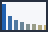
\includegraphics[width=0.5\linewidth]{figures/residuals.png}
  \caption{Residual norms $\norm{\iter{k+1} - \iter{k}}$ against the iteration
  index $k$, drawn rather than computed.}
  \label{fig:residuals}
\end{figure}

\subsubsection{A remark on indices}
\label{sec:indices}

The index $k$ counts iterations and the index $i$ counts coordinates.  We have
seen manuscripts in which this convention is reversed \cite{stand2019}; we do
not recommend the practice, but we note it here so that a
\texttt{subsubsection} exists.
